
\chapter{Experimental Studies}  \label{studies}
To evaluate our approach, we have implemented a tool, and conducted three empirical studies on a set of logged Java methods (LJMs) extracted from a real-world software system. In this section, we describe our experimental setup, present our studies, and discuss the results. 

\section{Experimental Setup}  \label{experimental_setup}
Our tool is a a plug-in to the Eclipse integrated development environment (IDE) that implements our algorithm. The tool consists of three main components: a correspondence tool, an antiunifier-building tool, and a clustering tool. The correspondence tool inputs a pair of LJMs, uses the Jigsaw framework to determine potential correspondences between their AST nodes, and outputs the generated CASTs and the Jigsaw similarity between them. The antiunifier-building tool inputs a pair of LJMs, applies our anti-unification algorithm to construct an anti-unifier with a special attention to logging calls, and outputs the detailed view of anti-unifier and similarity measure (as described in Section~\ref{meth-antiUnifier}). The clustering tool inputs a set of LJMs, applies a hierarchical clustering algorithm to classify them based on the similarity measurement, and outputs the detailed view of the generated anti-unifier for each cluster (as described in Section~\ref{meth-clustering}). 
% figure of architecture?

As a subject for our studies, we use \name{jEdit}, a programmer’s text editor tool written in Java programming language. We chose this subject because it is a real program that has been used constantly by many developers, and it makes real usage of logging calls.
Our tool extracts all LJMs within the source code of this program. However, a subset of them was selected containing 9 LJMs that showed varying levels of similarity on manual examination and has been used as a test suite throughout this study (see Table~\ref{table:ljms}). The org.gjt.sp.jedit.EditBus.send(...) method contains two logging calls. Therefore, we split it into two cases: case 3 contained the first logging call while the second one was removed; case 4 that only contained the second logging call. The last three LJMs were manually modified by adding some statements for the sake of dealing with important cases that we otherwise would have missed testing. Case 8 simulates an addition of an \code{if- }statement that formed a nested \code{if- }statement enclosing a logging call. Cases 9 and 10 simulate the addition of some statements to improve the test coverage.
We only used one test suite in this study, while different test suits may generate different results.


\begin{figure} [H]
  \centering
  \begin{tabular}{|c|l|c|}
    \hline
    Case & Logged Java methods & Size(LOC)\\
    \hline
    1& org.gjt.sp.jedit.PluginJAR.generateCache() &104\\   
   \hline
    2& org.gjt.sp.jedit.MiscUtilities.isSupportedEncoding(...) &9\\   
   \hline
    3& org.gjt.sp.jedit.EditBus.send(...) &14\\   
   \hline
    4& org.gjt.sp.jedit.EditBus.send(...)* &14\\   
   \hline
    5& org.gjt.sp.jedit.EditAction.Wrapper.actionPerformed(...) &5\\   
   \hline
    6& org.gjt.sp.jedit.EBPlugin.handleMessage(...) &6\\   
   \hline
    7& org.gjt.sp.jedit.BufferHistory.RecentHandler.doctypeDecl(...) &3\\   
   \hline
    8& org.gjt.sp.jedit.JARClassLoader.loadClass(...) &32\\   
   \hline
    9& org.gjt.sp.jedit.io.VFS.DirectoryEntry.RootsEntry.rootEntry(...) &36\\   
   \hline
    10& org.gjt.sp.jedit.ServiceManager.loadServices(...) &20\\   
    \hline
  \end{tabular}
  \caption{Logged Java methods used as our test suit; all are contained in the \name{org.gjt.sp.jedit} package.}
  \label{table:ljms}
\end{figure}

\section{Study 1: Jigsaw}  \label{study1}
The goal of study 1 is to assess how Jigsaw could effectively help us in determining potential correspondences and measuring similarity between Java elements of our test suite. 
We have implemented the correspondence tool, which uses the \name{JDT} framework to extract ASTs of a pair of LJMs and applies the \name{Jigsaw} framework to generate correspondence connections between their AST nodes and measure the similarity between them as explained in Section~\ref{Jigsaw}. 

\subsection{Setup}  \label{study1-setup}
The correspondence tool was used to compare LJMs of our test suite in a pairwise manner (55 test cases in total, including self-comparisons) and produce the CASTs of each pair. The Jigsaw similarity was also measured for each of these test cases.
We examined the generated CASTs of these test cases and selected a subset of 4 cases with various levels of correspondences as depicted in the Table~\ref{jigsaw_4_test_cases}. Case 1 contains the comparison of a Java element with itself. Case 2 contains the comparison of two Java elements that are both syntactically and semantically dissimilar.  Case 3 contains the correspondence between two Java elements that are syntactically dissimilar but are semantically relevant. Case 4 contains the comparison of a logging call with another Java element that is not logging call but is syntactically relevant.

\subsection{Results}  \label{study1-results}
The results of the pairwise comparison between LJMs of the test suite is visualized in Figure~\ref{fig:jigsaw_graph}. As it is shown, the jigsaw similarity for all self-comparisons is 1, while  the level of Jigsaw similarity is different for pairs containing distinct LJMs as our manual examination.

\begin{figure} [H]
  \centering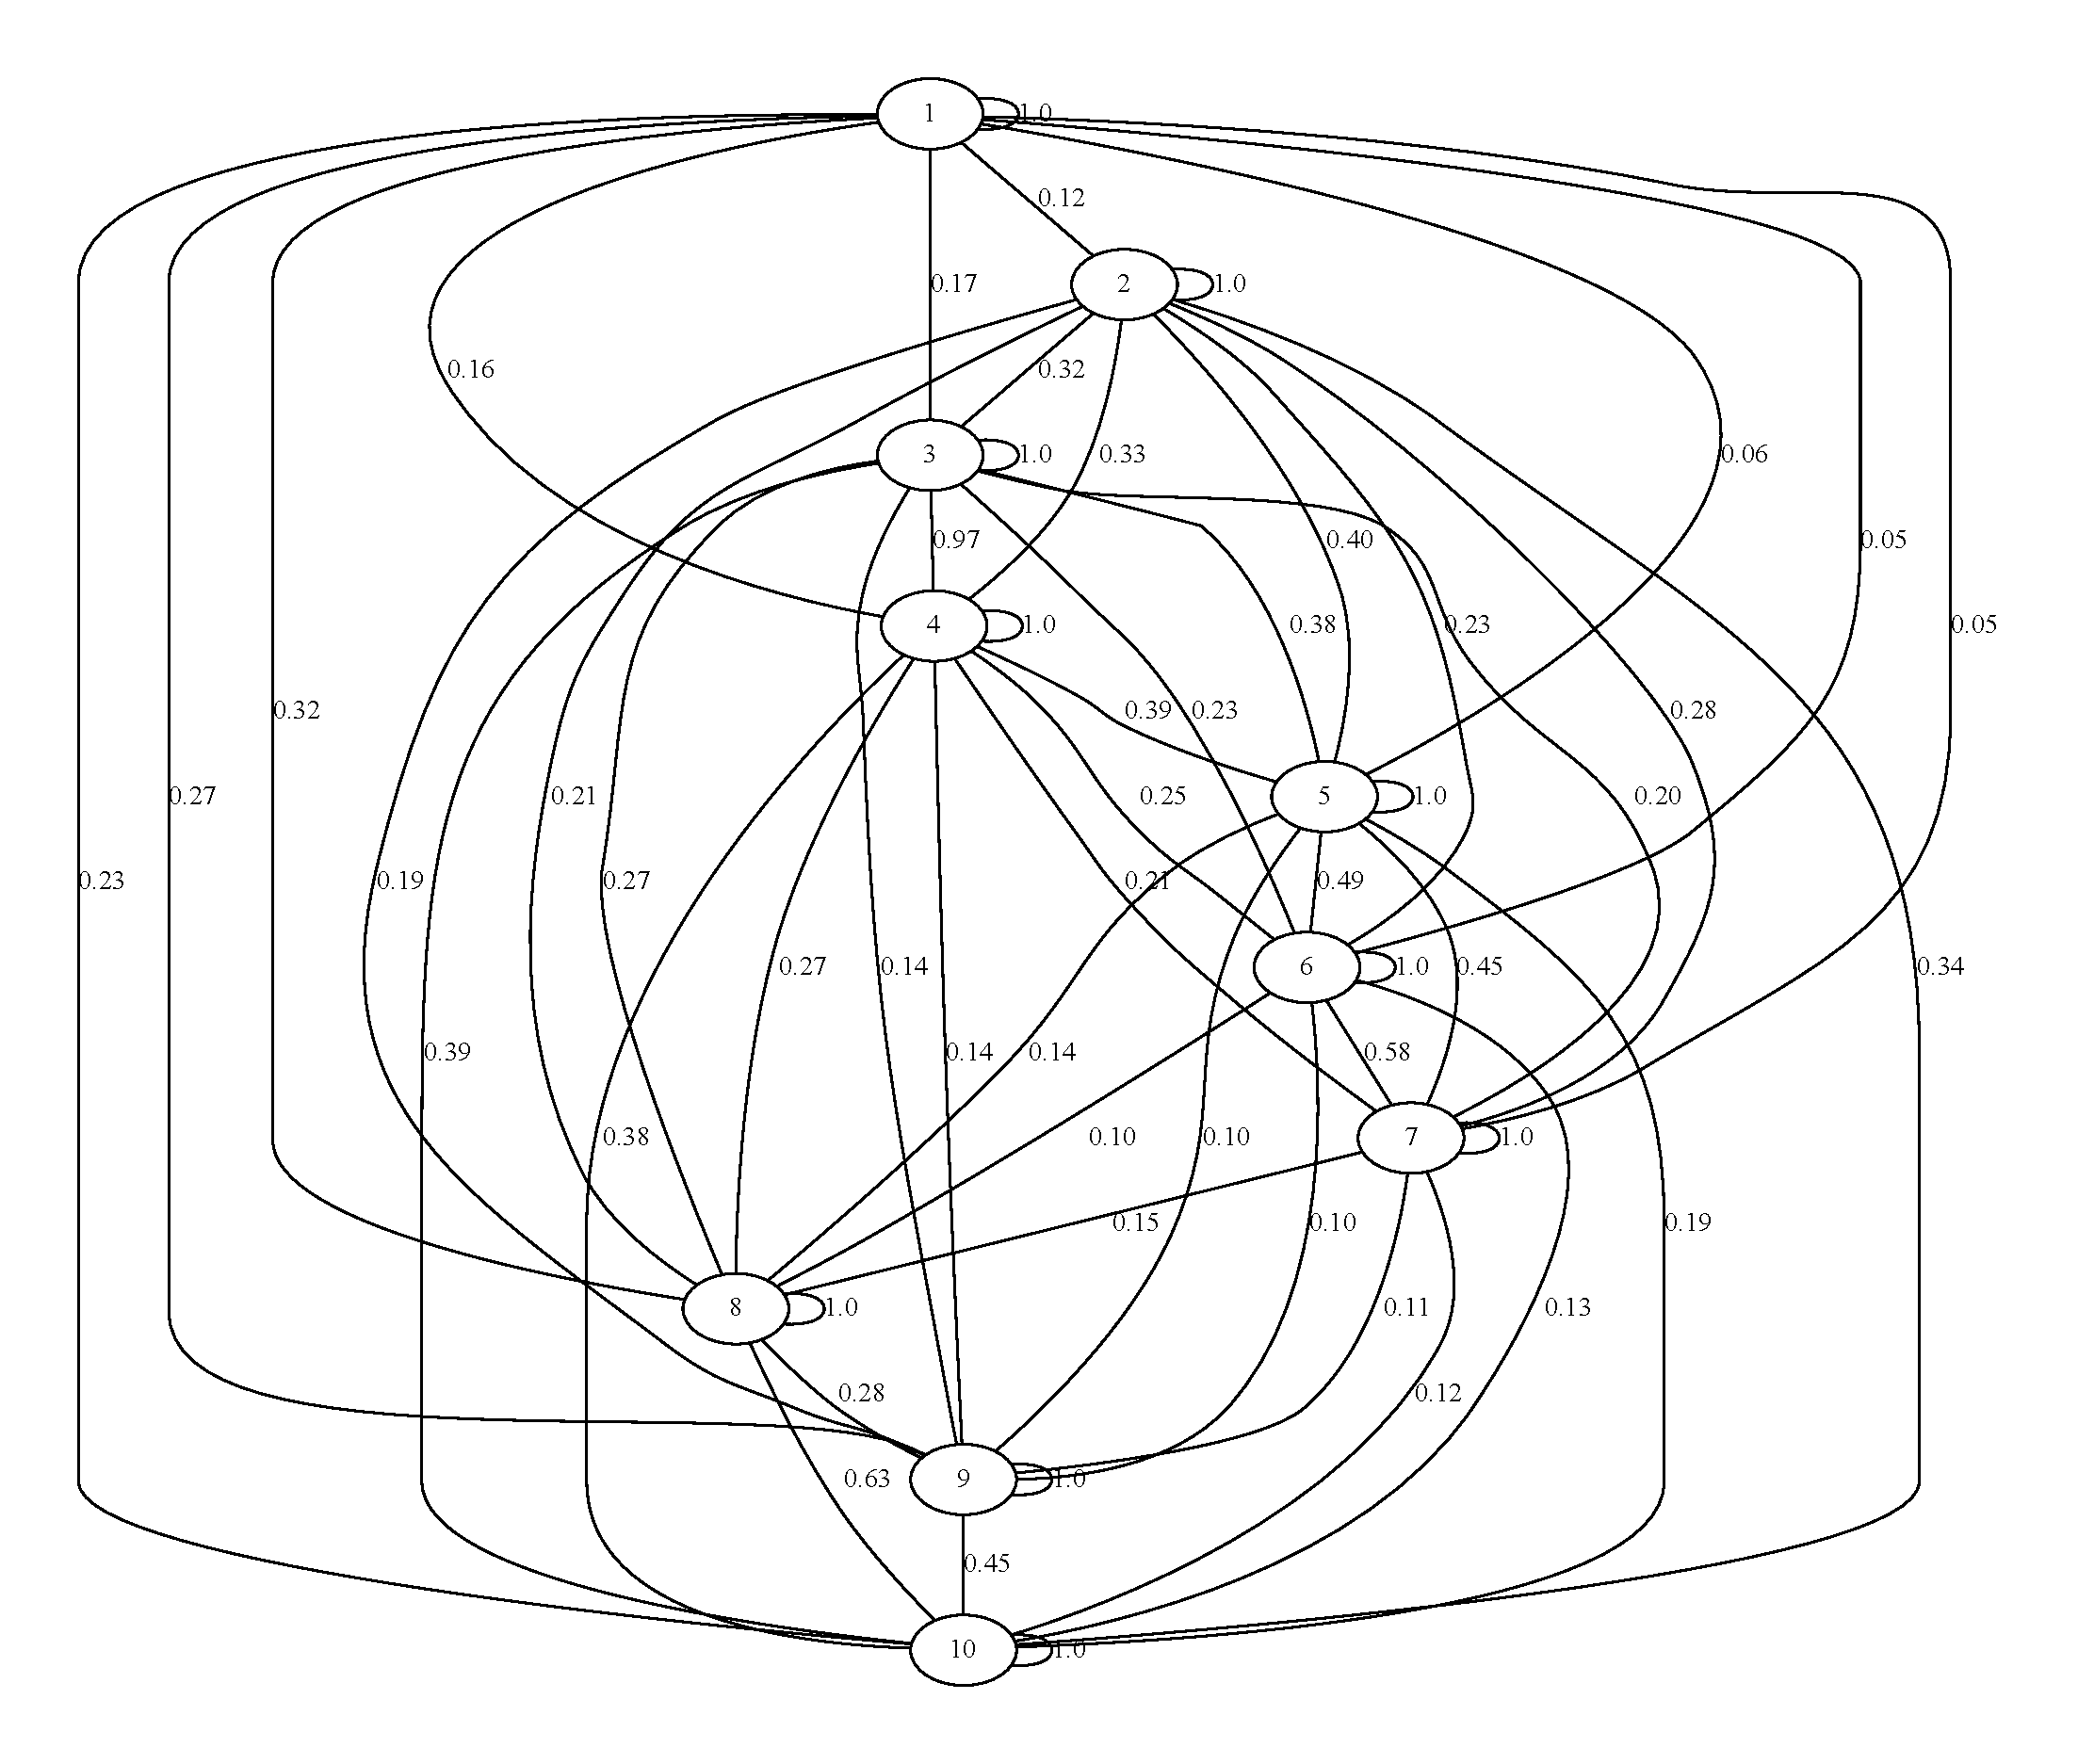
\includegraphics [width = \textwidth]{graphviz/jigsaw.pdf}
  \caption{A similarity graph representing pairwise Jigsaw similarities between LJMs shown in Table~\ref{table:ljms}.}
  \label{fig:jigsaw_graph}
\end{figure}


The analysis of the 4 test cases are shown in Table~\ref{jigsaw_4_test_cases}. Test Case 1 shows that a Java element that is compared with itself has a Jigsaw similarity of 1. Test Case 2 indicates that no correspondence connection is created when a Java element is compared with another Java element that is utterly dissimilar. Test Case 3 indicates that the similarity between a \code{for-} statement and a \code{while-} statement is non-zero and Jigsaw is able to detect semantic correspondences between Java elements. Test Case 4 shows that a logging call has non-zero similarity with another Java element that is not a logging call but is syntactically relevant. This case was handled by the antiunifier-builder tool via the removal of this kind of correspondence connection as described in  Section~\ref{meth-constraints}. 

\begin{figure}
  \centering
  \begin{tabular}{|c|l|c|}
    \hline
    Test case & Java source code fragment & Jigsaw Similarity\\
    \hline
    
    \multirow{2}{*}{{1}}&Log.log(Log.WARNING,this,"Unknown action: " + actionName);& \multirow{2}{*}{1}\\
    \cline{2-2}
                         &Log.log(Log.WARNING,this,"Unknown action: " + actionName);\\
    \hline
    
       \multirow{2}{*}{2}&return entry& \multirow{2}{*}{ No correspondence connection}\\
    \cline{2-2}
       &int i=0;\\
    \hline
  
    
 \multirow{2}{*}{3}&
 for (int i=0; i < comps.length; i++) {...} \\
  

    \cline{2-2}
      & 
while (entries.hasMoreElements())  { ...}    
      \\
    \hline    
    
    \multirow{2}{*}{4}&Log.log(Log.WARNING,this,"Unknown action: " + actionName);& \multirow{2}{*}{0.33}\\
    \cline{2-2}
      &EditBus.removeFromBus(this);\\
    \hline
    
  \end{tabular}
  \caption{Results from examining the Jigsaw similarity for 4 sample Java source code fragment pairs.}
  \label{jigsaw_4_test_cases}
\end{figure}
 


\section{Study 2: Detailed anti-unifier view}  \label{study2}
The goal of study 2 is to assess the effectiveness of our anti-unification algorithm for our test suite. We have implemented the antiunifier-building tool, which is developed atop the correspondence tool, based on the algorithm proposed in Section~\ref{meth-antiUnifier}. 

\subsection{Setup}  \label{study2-setup}
In this study, we manually attempted to create the detailed anti-unifier view for each pair of LJMs in the test suite (55 test cases in total). We first identified corresponding and non-corresponding Java elements for each LJM pair with a focus on preventing the correspondence of logging calls with anything else and then represented the anti-unifier in the detailed view (i.e., formatted as in Figure~\ref{}). We also computed the ratio of common Java elements in the detailed anti-unifier view to total number of Java elements of the two LJMs to measure the similarity.  
We also ran the antiunifier-building tool on each pair of LJM to construct the detailed anti-unifier view for each pair with a special attention to logging calls and to measure the similarity between the two LJMs. Furthermore, we used \name{Eclemma}, which is a Java code coverage tool for Eclipse, to measure the test coverage. Test coverage is defined as a measure of the completeness of the set of test cases. 


%The view would be in the form depicted in ..

\subsection{Results}  \label{study2-results}
We present the results of our analysis for a subset of 10 test cases (see Table~\ref{study2_test_cases}) in Table~\ref{study2_test_cases_results}. The analysis of the output has been divided into two categories: correspondence and similarity. "Correspondence" refers to the number of corresponding lines-of-code (LOC) detected by our tool that were found to be corresponded by our manual examination as well, and the number of LOC detected as corresponded by our tool but were not found to be corresponded in our manual inspection. We also present the percentage of the correct corresponding LOC to the total number of LOC of the two LJMs. "Similarity" refers to the similarity that is computed based on the the detected correspondences. It is calculated using both our tool and manual experiment.


In test case 8, \name{rootEntry} method contains a nested \code{if- }statement enclosing a logging call and \name{actionPerformed} method contains an \code{if-} statement enclosing another logging call. The analysis showed that a correct correspondence was detected between the inner \code{if- }statement inside the nested \code{if} and the single \code{if-} statement. Test cases 3 and 10 contains statements that are not found to be corresponded by our tool even though correspondences exist. For example, in test case 3, \name{isSupportedEncoding} method contains an assignment statement enclosed by an \code{if-} statement that does not have any correspondences and \name{send} method contains another assignment statement inside a \code{for-} statement without any correspondences as well. However, no correspondence was detected between the two assignment statements since their parent node are not corresponded.    



\begin{figure}
  \centering
  \begin{tabular}{|c|l|}
    \hline
    Test case & Logged Java methods \\
    \hline
    
    \multirow{2}{*}{{1}}&org.gjt.sp.jedit.PluginJAR.generateCache()\\
    \cline{2-2}
                         &org.gjt.sp.jedit.PluginJAR.generateCache()\\
    \hline
  
    \multirow{2}{*}{2}&org.gjt.sp.jedit.PluginJAR.generateCache()\\
    \cline{2-2}
                         &org.gjt.sp.jedit.EditBus.send(...)*\\
    \hline
    \multirow{2}{*}{3}&oorg.gjt.sp.jedit.MiscUtilities.isSupportedEncoding(...)\\
    \cline{2-2}
                         &org.gjt.sp.jedit.EditBus.send(...)\\
    \hline
    \multirow{2}{*}{4}&org.gjt.sp.jedit.EditBus.send(...)\\
    \cline{2-2}
                         &org.gjt.sp.jedit.EditBus.send(...)*\\
   \hline
   \multirow{2}{*}{5}&org.gjt.sp.jedit.EditBus.send(...)*\\
   \cline{2-2}
                         &org.gjt.sp.jedit.EditAction.Wrapper.actionPerformed(...)\\
 \hline
    \multirow{2}{*}{6}&org.gjt.sp.jedit.EditBus.send(...)*\\
   \cline{2-2}
                         &org.gjt.sp.jedit.BufferHistory.RecentHandler.doctypeDecl(...)\\
 \hline
    \multirow{2}{*}{7}&org.gjt.sp.jedit.EditAction.Wrapper.actionPerformed(...) \\
    \cline{2-2}
                         &org.gjt.sp.jedit.JARClassLoader.loadClass(...)\\
 \hline
    \multirow{2}{*}{8}&org.gjt.sp.jedit.EditAction.Wrapper.actionPerformed(...) \\
    \cline{2-2}
                         &org.gjt.sp.jedit.io.VFS.DirectoryEntry.RootsEntry.rootEntry(...)\\
 \hline
    \multirow{2}{*}{9}&org.gjt.sp.jedit.PluginJAR.generateCache()\\
    \cline{2-2}
                         &org.gjt.sp.jedit.BufferHistory.RecentHandler.doctypeDecl(...)\\
 \hline
    \multirow{2}{*}{10}&org.gjt.sp.jedit.io.VFS.DirectoryEntry.RootsEntry.rootEntry(...)\\
    \cline{2-2}
                         &org.gjt.sp.jedit.ServiceManager.loadServices(...) \\
  \hline
 
  \end{tabular}
  \caption{10 sample logged Java method pairs used as test cases.}
  \label{study2_test_cases}
\end{figure}


 
\begin{figure}
  \centering
  \begin{tabular}{|c|c|c|c|c|c|}
    \hline
    \multirow{2}{*}{Test case}&\multicolumn{2}{c|}{Correspondence}&\multicolumn{2}{c|}{Similarity}\\
    \cline{2-5}
    &Correct (\%)&Incorrect&human&tool\\
    \hline
    1&104(100)&0& 1.0 & 1.0\\
    \hline
    2&8(100)&0& 0.13& 0.13\\
    \hline
    3&6(85)&1&0.19& 0.16\\
    \hline
    4&4(100)&0&0.29 &0.29\\
    \hline
    5&5(100)&0&0.21 &0.21\\
    \hline
    6&3(100)&0&0.2 &0.2\\
    \hline
    7&5(100)&0&0.11 &0.11\\
    \hline
    8&7(100)&0& 0.1&0.1\\
    \hline
    9&3(100)&0&0.03&0.03 \\
    \hline
    10&14(87)&2&0.27 &0.22\\
    \hline
   
  \end{tabular}
  \caption{Results of constructing anti-unifiers with a focus on logging calls for the 55 test cases.}
  \label{study2_test_cases_results}
\end{figure}
 
The results of the pairwise comparison between LJMs of the test suite is visualized in Figure~\ref{fig:au_graph}. Our antiunifier-building tool succeeded in detecting correspondences with a special attention to anti-unifying logging calls and calculating pairwise similarities in 48 out of 55 test cases. In addition, the test coverage of our test cases was measured 82\% using \name{EclEmma}.

\begin{figure} [H]
  \centering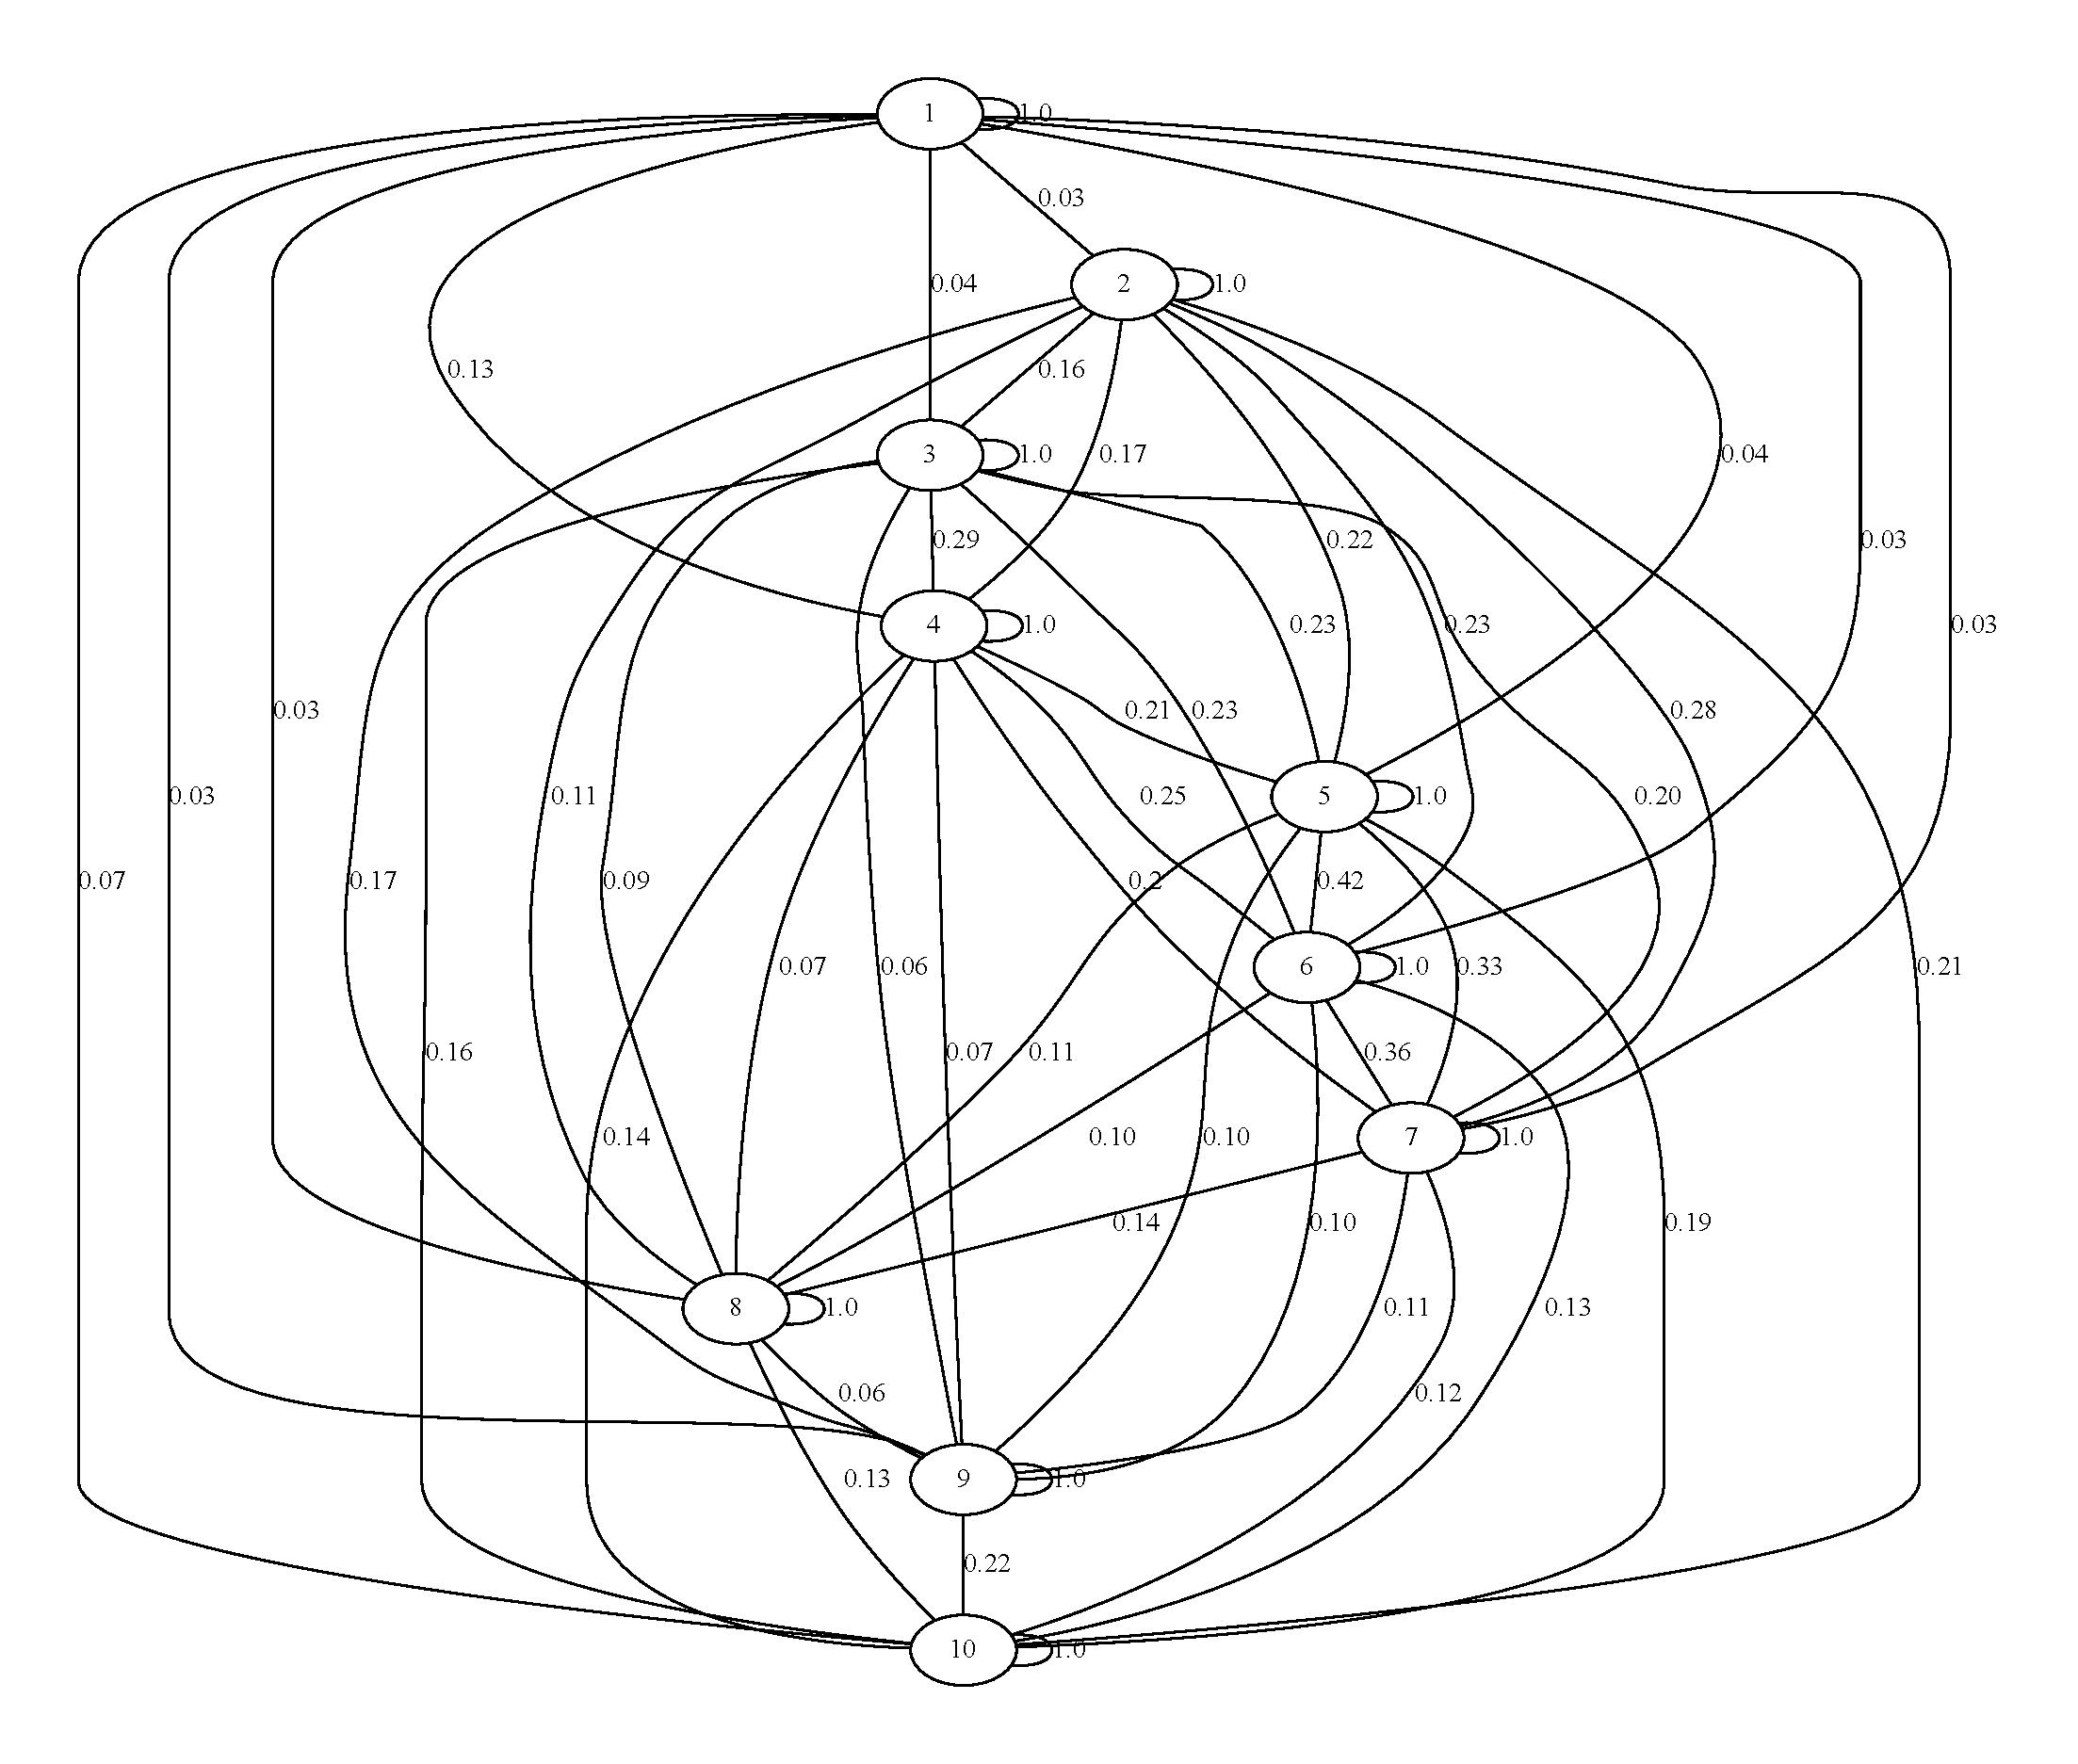
\includegraphics [width = \textwidth]{graphviz/au.pdf}
  \caption{A similarity graph representing pairwise similarities calculated by our tool between LJMs shown in Table~\ref{table:ljms}.}
  \label{fig:au_graph}
\end{figure}

\section{Study 3: Clustering}  \label{study3}
The goal of study 3 is to assess the effectiveness of our clustering algorithm for our test suite. We have implemented the clustering tool, which is developed atop the antiunifier-building tool, based on the hierarchical clustering algorithm proposed in Section~\ref{meth-clustering}.


\subsection{Setup}  \label{study3-setup}
We manually attempted to perform the hierarchical clustering on the set of LJMs from the test suite and constructed the detailed anti-unifier view for each cluster. Anti-unifiers were discarded when the anti-unification of LJMs does not allow the anti-unification of logging calls with one another as the Java elements enclosing them were not found to be corresponded. We also measured the level of similarity between LJMs in each cluster by computing the ratio of common Java elements in the detailed anti-unifier view to total number of Java elements of all LJMs in that cluster. We also ran the clustering tool on the set of LJMs to classify them using the similarity measurement.

\subsection{Results}  \label{study3-results}
We present the results of our analysis in Table~\ref{results_clustering}. The analysis of the output has been divided into three categories: correspondence, similarity, and relevancy. The analysis of "correspondence" and "similarity" was described in Section~\ref{study2-results}. "Relevancy" refers to the number of LJMs in each cluster that are detected to be relevant as their logging calls can be anti-unified with one another and cannot be anti-unified with logging calls of LJMs in the other clusters.
%AUASTs of all LJMs in each cluster

\begin{figure}
  \centering
  \begin{tabular}{|c|c|c|c|c|c|c|c|}
    \hline
  
    \multirow{2}{*}{Cluster}&\multicolumn{2}{c|}{Correspondence}&\multicolumn{2}{c|}{Similarity}&\multicolumn{2}{c|}{Relevancy}\\
    \cline{2-7}
    &Correct (\%)&Incorrect&human&tool&human&tool\\
    \hline
    1&28(100)&0&0.09&0.09  &4&4\\
    \hline
    3&24(92)&2&0.19&0.2& 3&3\\
    \hline
      2&9(100)&0&0.25&0.25& 3&3\\
 	\hline
  \end{tabular}
  \caption{Results from applying the clustering tool to the test suite.}
  \label{results_clustering}
\end{figure}

Our clustering tool succeeded in detecting the relevancy between LJMs of our test suite. It also successfully calculated the similarity between LJMs of 2 clusters out of 3. In cluster 2, the error in detecting correspondences was originated form the previous study and propagated to the clustering study. However, it is trivial (0.01) and would have a low impact in our final results.
